\documentclass[12pt, letterpaper]{article}

\usepackage{amsfonts}
\usepackage{amsmath} % needed for including equations
\usepackage[margin=1in]{geometry} % sets the margins to 1in
\usepackage{graphicx} % needed for figures
\graphicspath{{./figures/}} % allows figures to be placed in a different folder
\usepackage[hang,small,bf]{caption} % sets the style on the figure captions
\usepackage{epstopdf} % converts eps files to pdf to display in the latex document



\begin{document}

\begin{titlepage}

\begin{center}

\vspace*{\fill}

\vspace{0.5in}

% Insert your title here
{ \LARGE \bfseries Title of Your Prospectus}\\[.25in]

\large
by\\[.25 in]
% Change your name here
Andrew Tagg \\[1in]

A prospectus submitted to the faculty of\\
Department of Mechanical Engineering\\
Brigham Young University

\vspace{1in}

\today

\vspace*{\fill}

\end{center}

\end{titlepage}

\thispagestyle{empty}

\begin{center}
\vspace*{\fill}

\begin{figure}[htbp] %  figure placement: here, top, bottom, or page
   \centering
   
\includegraphics[width=2.5in]{byume_logo_clear.jpg} 
\end{figure}

\vspace{0.5in}

\Large{Prospectus Approval}\\[0.5in]

\end{center}

\hspace*{.47in}
\begin{minipage}[c]{5.25in}

\normalsize

Prospectus submitted by:

\vspace{.5in}

\makebox[2in]{\hrulefill} \hspace{1in} \makebox[2in]{\hrulefill}

% Change your name here
\parbox[b]{3in}{Andrew Tagg} \, Date
\vspace{0.5in}

This prospectus has been approved by each member of the Graduate Committee:
\vspace{0.5in}

\makebox[2in]{\hrulefill} \hspace{1in} \makebox[2in]{\hrulefill}

\parbox[b]{3in}{Committee Member - Chair} \, Date
\vspace{0.4in}

\makebox[2in]{\hrulefill} \hspace{1in} \makebox[2in]{\hrulefill}

\parbox[b]{3in}{Committee Member} \, Date
\vspace{0.4in}

\makebox[2in]{\hrulefill} \hspace{1in} \makebox[2in]{\hrulefill}

\parbox[b]{3in}{Committee Member} \, Date

\end{minipage}

\vspace*{\fill}

\pagebreak

\setcounter{page}{1}

%What are you trying to do? Articulate your objectives using absolutely no jargon.
%How is it done today, and what are the limits of current practice?
%What is new in your approach and why do you think it will be successful?
%Who cares? If you succeed, what difference will it make?
%What are the risks?
%How much will it cost? (this is less relevant for a prospectus)
%How long will it take?
%What are the mid-term and final “exams” to check for success?

\section{Problem Statement}

% What’s wrong with the world right now
    % High fidelity unsteady aerodynamic modeling is needed but too expensive for practical applications in optimization and control
    % Highlight eVTOL as an example



% Set the stage ("Who cares")
High fidelity aerodynamic modeling is an essential tool in the analysis of modern aircraft, yet its use in applications such as design optimization and real time control is severely limited due to high computational costs.  Instead, current optimization and control loops mainly rely on simplified, steady state aerodynamic models which are desirable for rapid evaluation, but neglect essential characteristics of unsteady flight. If we can overcome the computational hurdle, and incorperate high fidelity, unsteady aerodynamics into our design and control algorithms, we can significantly improve the performance, safety, and reliability of next-generation aircraft systems. 

% State the theme - your solution
In this work, we propose a framework to fully incorporate high fidelity aerodynamics into optimization and control loops through an unsteady vortex particle method (VPM).  We will accelerate VPM simulation with a novel deep learning technique designed to reduce the number of time steps required to solve the governing differential equations.  This will significantly reduce computational cost, thereby enhancing the practicality of the VPM in large scale iterative optimization.  For real time control, we will leverage Koopman operator theory to learn linear representations of VPM dynamics, and develop methods to improve the generalizability of the Koopman learning process.  By learning linear representations of the underlying flow dynamics, we will support rapid and accurate control synthesis using tried and true linear techniques.

% Create a vision ("So what")
By developing these key innovations, we will enable large scale integration of VPM aerodynamics into the design and control process.  High fidelity aerodynamics will inform decisions from early conceptual design all the way through to the flight control stage.  These decisions will not only consider how the aircraft behaves, but also how the surrounding air moves and evolves during complex maneuvers.  With these enhaced modeling capabilities available during moments of crucial decision making, we will open the door for aircraft that are not only more efficient and capable, but fundamentally more intelligent in how they interact with their environment. 

\section{Background}


The next generation of aircraft systems is being conceved to operate in increasingly challenging conditions, and execute mission profiles that span multiple diverse flight regimes.  Some aircraft are capable of morphing their wings to access the post stall region for precision landings \cite{bakhshi2025coupled}.  Other biologically inspired vehicles replicate nature and achieve remarkable agility \cite{lee2022transition, tian2020cfd}.  Electric vertical takeoff and landing (eVTOL) aircraft employ lifting propulsors and fixed wing components to takeoff in hover and then transition to cruise.  

All of these aircraft pose significant operational challenges, because they must undergo complex dynamic maneuvers in which unsteady aerodynamics play a leading role.  For example, the eVTOL transition from hover to cruise is largely characterized by wake mixing, and unsteady interactions between propellers and lifting surfaces that are difficult to predict.  In the presence of strong unsteady loading, the aircraft must execute a series of complex control inputs that balance forward motion with vertical propulsion while simultaneously managing rotation. In addition, successful transitions often require adherence to constraints on power \cite{moradi2024urban}, acceleration \cite{xiang2024autonomous}, acoustic output \cite{raza2025noise}, and obstacle avoidance \cite{shukla2025trajectory}. Considering all of these factors at once quickly becomes an overwhelming task for a pilot.

The key to navigating this complex space of decisions is trajectory optimization, which is the process of optimizing the path, and control inputs of the maneuver to minimize some desired objective subject to required constraints.  Recent work in eVTOL trajectory optimization has exposed key insights that highlight the importance of consdering complex aerodynamic phenomena when optimizing these transition maneuvers.  \cite{chauhan2020tilt} optimized the takeoff trajectory of a tilt-wing aircraft, and found that optimal trajectories involve operating at or near the stall region.  This was complemented by other work which investigated the possibility of using active flow control to delay stall during a tilt-wing transition \cite{panish2025tiltwing}. Another study directly implemented a constraint to avoid the vortex ring state during takeoff and landing and showed how this constraint afffected the optimal path \cite{park2023trajectory}.

Considering these unsteady aerodynamic phenomena during trajectory optimization is crucial for safe and optimal performance, and therefore affects overall aircraft design decisions.  Recent work has shown that trajectory optimization plays a key role in battery sizing \cite{liu2024flight}, and can inform airfoil design \cite{panish2025tiltwing}.  This is why several design studies have directly incorperated the trajectory into the optimization process \cite{sarojini2023large, kaneko2024simultaneous, kaneko2025simultaneous}. 

One of the most important results of trajectory optimization is it's natural application to automation and control.  Classical control methods often rely on linear models that are only valid locally, and cannot be simultaneously applied to the entire flight envelope of a modern transitioning vehicle.  Instead, many efforts have employed trajectory optimization as a planning process to develop controllers that evolve over time through gain scheduling \cite{thompson2020robust}, or onboard control policy updates \cite{gupta2025realtimeplanningcontrolvortex}.

Notably, there are approaches that allow for the use of a single control policy for the entire transition.  These either employ advanced robust control strategies such as $H^{\infty}$ methods \cite{yang2021robust}, or rely on Koopman operator theory to learn globally linear dynamic representations \cite{korda2018koopman, abraham2017modelbased, zinage2021koopman}.  Koopman operator theory presents an especially promising option because it provides a way to learn dynamics that are linear everywhere in the state space, thus opening the door for linear controllers that are accurate and can be applied in any flight regime without sacrificing performance.  The main limitation preventing the widespread use of current Koopman methods is that they require exhaustive data to be completely general, which is difficult to obtain for high dimensional or high fidelity problems. 

The large foundation of work in trajectory optimization and control of aircraft which undergo complex transition maneuvers represents a robust and versitile framework for performing optimization and control across multiple flight regimes.  This existing work has exposed critical design tradeoffs for these types of aircraft, and higlighted the importance of considering time varying dynamics during the transition phase.  

However, the main limitation of the current base of research is that nearly all of these studies rely heavily on overly simplified aerodynamic models, which either assume steady state flow, or other idealizations that are not accurate during an unsteady maneuver.  This is a real problem because there is strong evidence to suggest that model fidelity has a severe effect on the outcome of trajectory optimization \cite{anderson2021acomparison}.  Some studies have directly compared steady state models with unsteady models during an eVTOL transition and found significant discrepancy \cite{tagg2024trajectory}.  Others have quantified the effect of unsteady aerodynamics during rotational motion, and found that it greatly impacts the dynamic stability of the aircraft \cite{wang2012unsteady}.  Clearly, unsteady aerodynamics play an important role during the transition of these aircraft, and cannot be justifiably ignored during analysis and optimization. 

Some effort has been made toward improving model fidelity in optimization and control applications.  One common approach is to generate high fidelity CFD data, and then tune the parameters of the low fidelity model \cite{dean2008aircraft, tian2020cfd, gortz2007towards}.  This is definitely an improvement because the new parameters are informed by high fidelity simulations, but unless the parameters are updated constantly, it is still subject to the limitations of a steady state model.  Other studies have focused on applying fast unsteady aerodynamic models like the harmonic balance method \cite{thomas2004modeling} and Theodorsen's theory \cite{bhoir2004output}.  While useful, these methods apply only to very simple oscillatory motions and cannot represent a more complex maneuver.  

The best effort so far to fully incorperate high fidelity simulations into optimization and control loops has come from a pair of studies that employed a light weight two-dimensional vortex particle method to trajectory optimization \cite{perrotta2023planningcontroldynamicmorphingwing} and then real time control \cite{gupta2025realtimeplanningcontrolvortex} for fixed wing perching maneuvers.  Even though these VPM models were limited to two dimensions, and under 100 particles, the studies showed improved performance and more accurate precision landings when the unsteady model was used.  This is direct evidence that employing high fidelity models in control loops can lead to better results, but the scope of these improvements is still very much limited by computational cost as demonstrated by the need for such a light weight version of the VPM.   

One promising alternative is the use of deep learning to capture unsteady fluid dynamics.  There have been many studies which apply vanilla neural networks \cite{collotta2014arealtime, sabater2021fast}, convolutional neural networks \cite{abucide2021adata, hwang2025aerodynamic}, and physics informed neural networks \cite{raissi2019physics, lin2025aphysics} to learn fluids flows or aerodynamic coefficients.  Other papers have attempted to learn high resolution flow fields from low resolution solutions \cite{sharma2025accelerating, gao2021super}, or focus on learning the underly dynamics of the system using neural ODEs \cite{jarry2025neuralodeapproachaircraft, ma2024development}.  These approaches offer a compelling solution to the problem of high fidelity optimization and control because they allow for rapid evaluation of the deep surrogate network at significantly reduced cost.  Despite the significant advancements in deep learning, existing data-driven approaches often struggle to generalize completely unless exhaustive training data are provided, which is extremely difficult in the high dimensional and computationally expensive world of CFD. 

Deep learning offers the potential for rapid evaluation and can capture unsteady aerodynamic effects, but traditional data-driven approaches often fail to generalize without prohibitively large datasets. Low-fidelity models are computationally efficient and generalize well, yet they neglect critical unsteady phenomena. High-fidelity simulations, on the other hand, are accurate and broadly applicable but are too computationally expensive for practical use in iterative optimization and real-time control. What is needed is a methodology that combines speed, accuracy, and generality, enabling unsteady aerodynamics to directly inform design and control decisions.

The proposed work addresses this challenge through a novel integration of high-fidelity simulation and deep learning. Rather than using data to fully replace the vortex particle method (VPM), we focus on accelerating the simulation of known VPM dynamics by reducing the number of required time steps. This approach will make VPM-based trajectory optimization significantly more feasible by reducing a primary bottleneck in VPM simulation. Building on this foundation, we will develop a method for learning Koopman linear representations that leverages known PDE solution methods and deep learning, enhancing generalizability across flow conditions. The resulting framework will enable real-time control informed by high-fidelity, unsteady aerodynamics, bridging the gap between computationally expensive simulations and practical optimization and control applications.


% introduce some cases where unsteady aero is imortant
% point to trajectory optimization as a natural solution to these challenges
% introduce studies on trajectory optimization showing that complex aircraft dynamics are important to consider
    % 1 tilt-wing takeoff ... operating near stall
    % 4 trajectory optimization for takeoff and landing ... vortex ring state 
    % 2 tiltwing eVTOL transition ... active flow control, airfoil design
% claim that these are important for safe maneuvering, but also important for optimal aircraft design
    % 2 flight analysis and optimization ... trajectory optimization informs battery sizing
    % 2 tiltwing eVTOL transition ... active flow control, airfoil design
% cite optimization studies that considered both trajectory and design, and highlight the need for considering dynamic maneuvers in aircraft design, not just steady state
    % 1 large-scale multidisciplinary ... subsystems, including trajectory ?
    % 3 simultaneous optimization ... co-design of both
    % 4 simultaneous optimization ... coupling methods
% explain that perhaps the most important use of trajectory optimization is it's natural application to automation and control.  
% point out that because unsteady transition have drastically changing dynamics, traditional control methods that rely on locally linear models fail, and we generally employ trajectory optimization to imform how our controllers must change with time through the maneuver
    % 1 modeling and control of transition ... gain scheduling lqr
    % 4 robust control ... lqr gain scheduling
    % 8 real-time planning and control ... 2D VPM used for onboard control policy updates
    % 6 control of an eVTOL using ... switching between controllers
% explain that other methods allow for a single control policy throughout the transition, which tends to lead to more robust and smooth performance
    % 5 robust full-envelope ... h-infinity for single controller
    % 1 linear predictors for nonlinear dynamic systems ... koopman and MPC
    % 4 extending the extended ... EDMD
    % 5 physics-informed koopman ... PIKN
% emophasize the promise of koopman methods because of it's ability to linearize a nonlinear dynamic system and generalize to all flight regimes without sacrificing performance like robust control theory.
% point out that current koopman implementations rely heavily on data, and are subject to overfitting unless exhaustive data are generated, which becomes difficult in high dimensions and high computational costs.
% highlight the important contributions of all of this work in delivering a robust and versitile framework for analyzing eVTOL transition maneuvers, and demonstrating that considering time varying dynamics is crucial for aircraft performance.
% state that nearly all of the current work in this field relies on overly simplified aerodynamic models, which rely on steady state, other simplifiying assumptions.
% Explain that this represents a real problem, because studies have shown that the fidelity of the aerodynamic model can severely affect the system's performance
    % 1 a comparison ... model comparisons
    % 2 trajectory optimization of eVTOL and conventional ... VPM vs VLM-BEMT
    % 7 planning and control ... 2D vpm for planning and control showed improved performance
    % 8 real-time planning and control ... 2D VPM used for onboard control policy updates
    % 8 unsteady aerodynamics modeling ... quantifying unsteady effects on dynamic stability
% show that some recent work has been directed toward improving the aerodynamic fidelity in optimization and control applications
    % 4 design-oriented computational ... passing derivatives through CFD
    % 5 modeling viscous ... harmonic balance method
    % 6 discrete adjoint ... harmonic balance method
    % 12 aircraft stability and control ... system id from CFD
    % 13 CFD-based parameter tuning ... tuning parameters from CFD
    % 14 towards an efficient ... stability and control derivatives from CFD
    % 9 output feedback nonlinear ... pitching wing control with unsteady aero
    % 7 planning and control ... 2D vpm for planning and control showed improved performance
    % 8 real-time planning and control ... 2D VPM used for onboard control policy updates
% point out that while these studies represent steps in the right direction, each one has limitations (do this in paragraph, not at the end)
% show that deep learning presents a promising approach due to it's remarkable ability to model physics, and has been extensively applied to aerodynamics and flight applications
    % 1 real-time prediction ... neural networks used to predict unsteady flows and coefficients
    % 2 a dataaugmentation ... CNN for CFD
    % 3 aerodynamic ... CNN for CFD
    % 4 fast predictions ... neural network training
    % 5 a neural ode approach ... neural ODE for flight dynamics
    % 6 development and implementation ... physics informed NODE
    % 7 accelerating cfd simulations ... super-reslution for adaptive mesh refinement
    % 8 super-resolution and denoising ... super-resolution for map from low fideliy to high fidelity
    % 10 physics-informed neural networks ... PINN paper
    % 11 a physics-informed ... PINN to learn parameters
    % 12 flight dynamics modeling using ... PINN to learn dynamics
% state that the main limitation of the current practice is that exhaustive data is required to generalize 

    

% summarize the main limitations
% state how the proposed work will fix those problems





% Trajectory optimization
    % 1 tilt-wing takeoff ... operating near stall
    % 2 tiltwing eVTOL transition ... active flow control, airfoil design
    % 4 trajectory optimization for takeoff and landing ... vortex ring state 
    % 6 trajectory optimization of eVTOL and conventional ... 
    % 10 coupled trajectory and aerostructural ... morphing wing improves performance

% Co-design of aircraft and trajectory
    % 2 flight analysis and optimization ... trajectory optimization informs battery sizing
    % 3 simultaneous optimization ... co-design of both
    % 4 simultaneous optimization ... coupling methods

% Design optimization
    % 1 large-scale multidisciplinary ... subsystems, including trajectory ?
    % 4 design-oriented computational ... passing derivatives through CFD
    % 5 modeling viscous ... harmonic balance method
    % 6 discrete adjoint ... harmonic balance method

% Control law design
    % 1 modeling and control of transition ... gain scheduling lqr
    % 4 robust control ... lqr gain scheduling
    % 5 robust full-envelope ... h-infinity for single controller
    % 6 control of an eVTOL using ... switching between controllers
    % 8 real-time planning and control ... 2D VPM used for onboard control policy updates
    % 9 output feedback nonlinear ... pitching wing control with unsteady aero
    % 12 aircraft stability and control ... system id from CFD
    % 13 CFD-based parameter tuning ... tuning parameters from CFD
    % 14 towards an efficient ... stability and control derivatives from CFD

% Effect of model fidelity on performance
    % 1 a comparison ... model comparisons
    % 2 trajectory optimization of eVTOL and conventional ... VPM vs VLM-BEMT
    % 7 planning and control ... 2D vpm for planning and control showed improved performance
    % 8 unsteady aerodynamics modeling ... quantifying unsteady effects on dynamic stability
    % some  papers in other sections also show this

% Machine learning
    % 1 physics constrained ... GAN used to reduce to a feasible space of trajectories
    % 3 performance modeling ... RBF used for modeling 
    % 4 deep reinforcement learning ... RL used for policy training
    
% Deep learning
    % 1 real-time prediction ... neural networks used to predict unsteady flows and coefficients
    % 2 a dataaugmentation ... CNN for CFD
    % 3 aerodynamic ... CNN for CFD
    % 4 fast predictions ... neural network training
    % 5 a neural ode approach ... neural ODE for flight dynamics
    % 6 development and implementation ... physics informed NODE
    % 7 accelerating cfd simulations ... super-reslution for adaptive mesh refinement
    % 8 super-resolution and denoising ... super-resolution for map from low fideliy to high fidelity
    % 10 physics-informed neural networks ... PINN paper
    % 11 a physics-informed ... PINN to learn parameters
    % 12 flight dynamics modeling using ... PINN to learn dynamics

% Koopman
    % 1 linear predictors for nonlinear dynamic systems ... koopman and MPC
    % 4 extending the extended ... EDMD
    % 5 physics-informed koopman ... PIKN

% Papers about VPM

% What have others tried
    % Using simplified aerodynamics
    % Using data driven techniques for faster models

% Literature review

% Limitations

\section{Research Objectives}

The central goal of this work is to facilitate the incorporation of high-fidelity, unsteady aerodynamics into optimization and control processes.  To accomplish this goal, we will focus on four primary research objectives.

\begin{enumerate}
    \item \textbf{Demonstrate VPM-based trajectory optimization for an eVTOL transition maneuver.} 
    We will apply the VPM to simulate unsteady aerodynamic effects during an eVTOL hover-to-cruise maneuver and use this model to optimize the transition trajectory. This objective will address practical challenges associated with VPM-based optimization, such as noise and convergence, and provide a baseline in terms of computation time for comparison against future VPM acceleration efforts.  Included in this study will be a comparison of high fidelity and low fidelity models and an analysis of their impact on the trajectory optimization.
    \item \textbf{Develop a methodology to accelerate VPM simulations by reducing the number of required time steps.} 
    By addressing a major computational bottleneck in VPM, this objective aims to make high-fidelity simulations fast enough to be used in iterative optimization. We will validate the method by quantifying the speedup and the accuracy of the accelerated VPM simulations. 

    \item \textbf{Develop a methodology to learn Koopman linear representations of VPM dynamics and improve generalizability.} 
    This objective will seek to uncover linear representations of VPM dynamics, enabling real time control synthesis informed by VPM aerodynamics.  We will apply a combination of physics informed deep learning, and PDE solution methods to demonstrate improved generality over state of the art approaches.  


    \item \textbf{Apply these new techniques to the eVTOL transition maneuver problem.}
    This objective will be an application of the novel techniques developed and will serve to demonstrate their effectiveness in the context of an eVTOL transition maneuver.  We will conduct trajectory optimization using the accelerated VPM simulations, and control synthesis using the learned Koopman operator.
\end{enumerate}

% What will you do
    % Demonstrate the need for high fidelity modeling during optimization, and the feasibility of applying it
    % Reduce simulation costs with neural networks
    % Learn linear representations for control


\section{Proposed Research}

% How will you do it
    % Trajectory optimization using VPM to demonstrate feasibility and need
    % Neural time step reduction to reduce cost
    % Method of characteristics to learn Koopman operators


% Summarize the high level approach
As outlined in the previous section, the proposed work will have four main thrusts.  First, the VPM will be applied to an eVTOL transition optimization problem to demonstrate feasibility of the optimization approach and highlight the need for high fidelity modeling in this case.  Next, the method of applying deep learning to accelerate VPM simulation through time step reduction will be developed and tested.  After successful VPM accelerations are achieved, the focus of the project will turn toward improving the generality of the Koopman learning problem, specifically for VPM dynamics.  Finally, these innovations will be utilized to optimize trjectories and perform active feedback control for the eVTOL transition maneuver to demonstrate improved performance and reduced computational cost.  

% Method subsections
\subsection{Trajectory optimization}

For trajectory optimization, we represent the aircraft as a set of dynamic states $\mathbf{x}$, and control inputs $\mathbf{u}$ and we express the discrete time evolution of the aircraft states as

\begin{equation}
    \mathbf{x}_{k+1} = F(\mathbf{x}_k, \mathbf{u}_k)
\end{equation}

where $k$ denotes the current time step, and $F$ is the function that advances the state to time step $k+1$.

We then formulate the following optimization problem

\begin{equation}
    \begin{matrix}
        \underset{\mathbf{x}_k, \mathbf{u}_k}{\text{minimize}} & \overset{N}{\underset{k=0}{\sum}} \mathbf{u}_k^T R \mathbf{u}_k \\ \\ 
        \text{subject to} & \mathbf{x}_{k+1} = F(\mathbf{x}_k, \mathbf{u}_k) \\
        & \mathbf{x}_0 = \mathbf{x}_{\text{init}} \\ 
        & \mathbf{x}_N = \mathbf{x}_{\text{des}}
    \end{matrix}
\end{equation}

The objective is a quadratic penalty on control effort that is determined by the weight matrix $R$.  The system must adhere to the discrete dynamic equations $\mathbf{x}_{k+1} = F(\mathbf{x}_k, \mathbf{u}_k)$, and it must start at a predetermined state $\mathbf{x}_{\text{init}}$ and end at a desired state $\mathbf{x}_{\text{des}}$.  Therefore solving this optimization problem will mean that the system successfully maneuvered to the desired location while expending the least ammount of control effort possible. 

This problem is highly nonlinear due to the system dynamics $F$, which include unsteady wake mixing from the VPM. To make the problem tractable, we construct a local linear approximation of the dynamics using a first-order Taylor series expansion:  

\begin{equation}
\label{eq:taylor_series}
    \mathbf{x}_{k+1} = F(\mathbf{x}_k,\mathbf{u}_k) \approx F(\mathbf{x}^*,\mathbf{u}^*) + A (\mathbf{x}_k - \mathbf{x}^*) + B (\mathbf{u}_k - \mathbf{u}^*)
\end{equation}

where $A$ and $B$ are the Jacobians of the $F$ with respect to the states and inputs, evaluated about a nominal point $(\mathbf{x}^*, \mathbf{u}^*)$.  For convenience, we rearrange and write


\begin{equation}
\label{eq:taylor_series}
    \mathbf{x}_{k+1} = A \mathbf{x}_k + B \mathbf{u}_k + C
\end{equation}

where $C = F(\mathbf{x}^*, \mathbf{u}^*) - A \mathbf{x}^* - B \mathbf{u}^*$

This now represents a linear approximation of the nonlinear dynamics, but it is only valid close to $\mathbf{x}^*$ and $\mathbf{u}^*$.  For an eVTOL transition, this is problematic because final desired state is cruise, which is very different from hover.  To remedy this, we update the linear model at every time step, and allow $A$, $B$ and $C$ to vary with time.  The equation now becomes


\begin{equation}
\label{eq:taylor_series}
    \mathbf{x}_{k+1} = A_k \mathbf{x}_k + B_k \mathbf{u}_k + C_k
\end{equation}

And the optimization problem becomes


\begin{equation}
    \label{eq:LQR}
    \begin{matrix}
        \underset{\mathbf{x}_k, \mathbf{u}_k}{\text{minimize}} & \overset{N}{\underset{k=0}{\sum}} \mathbf{u}_k^T R \mathbf{u}_k \\ \\ 
        \text{subject to} & \mathbf{x}_{k+1} = A_k \mathbf{x}_k + B_k \mathbf{u}_k + C_k\\
        & \mathbf{x}_0 = \mathbf{x}_{\text{init}} \\ 
        & \mathbf{x}_N = \mathbf{x}_{\text{des}}
    \end{matrix}
\end{equation}


Because this formulation features a quadratic objective and linear constraints, it is classified as a quadratic program (QP) and can be solved analytically.  However, the linear dynamics described by $A_k$, $B_k$, and $C_k$ are an approximation that is only valid close to the original trajectory that was used to construct the taylor series. If we use this model to solve the QP problem we will get an updated trajectory that is potentially different from the original one, and the model will no longer be valid.  Therefore, iteration is required to converge to the true optimal solution. The procedure to iteratively solve the full nonlinear optimization problem is as follows:  

\begin{enumerate}
    \item Provide an initial guess trajectory.  
    \item Linearize the dynamics at each point along the trajectory to obtain $A_k$, $B_k$, and $C_k$.  
    \item Solve the QP problem defined in \ref{eq:LQR} to obtain a new trajectory.  
    \item Repeat steps 2–3 until convergence is achieved.  
\end{enumerate}

This procedure allows us to solve arbitrary nonlinear trajectory optimization problems, but solving it in the VPM presents additional challenges that need to be overcome.  The main challenge associated with VPM-based trajectory optimization is derivative computation.  The jacobian matrices $A_k$ and $B_k$ are computed as


\begin{equation}
\label{eq:jacobians}
    A_k = \frac{\partial F}{\partial \mathbf{x}} \Big|_{\mathbf{x}_k^*, \mathbf{u}_k^*} \quad B_k = \frac{\partial F}{\partial \mathbf{u}} \Big|_{\mathbf{x}_k^*, \mathbf{u}_k^*}
\end{equation}

These derivatives are obtained via automatic differentiation (AD) by propagating derivatives through the VPM simulation, which is computationally expensive. The fine temporal resolution required in VPM often leads to simulations with thousands of time steps, further increasing the cost of derivative calculations along the trajectory.  

To reduce this computational burden, $A_k$ and $B_k$ are not computed at every time step. Instead, they are evaluated at a limited number of key points along the trajectory, exploiting the observation that the Jacobians typically change gradually as the aircraft transitions from hover to cruise.  

Once $A_k$ and $B_k$ have been calculated at these select points, the missing values at intermediate time steps are estimated by fitting a curve using least-squares regression.  This approach substantially reduces the number of derivative computations required, thereby lowering overall computational cost. 

%\begin{figure}[hbt!]
%\centering
%\includegraphics[width=0.7\textwidth]{figures/derivative_regression.png}
%\caption{}
%\label{fig:derivative_regression}
%\end{figure}


Another challenge presented by the VPM is the fact that the linear model matrices $A_k$, $B_k$, and $C_k$ are generally very noisy.  This noise is inherant in an unsteady aerodynamic model because vortical structures in the flow are shed from rotors that are spinning at a very high RPM. The high blade passage frequency causes rapidly oscillating unsteady forces, which is completely consistent from a physics stand point, but nonetheless causes numerical issues for the optimization and makes it difficult to achieve convergence. 

In order to improve the numerical performance of the optimization, we seek to filter out the high frequency content of the VPM.  This is partly achieved through the regression of the derivative values described previously - fitting a relatively low order curve to the values $A_k$ $B_k$, and $C_k$ ensures a smooth progression in time.  However, there is still a significant ammount of noise in these matrices across optimization iterations, which causes irregular optimizer steps, and hinders convergence.

To address this, we apply an exponential moving average of the matrices to smooth out the noise from iteration to iteration

\begin{equation}
\label{eq:EMA}
    \bar{A}_k = \alpha A_k + (1 - \alpha) \bar{A}_k
\end{equation}

where $\bar{A}_k$ is the tracked average of the derivatives across iterations, $A_k$ is the newly computed derivative, and $\alpha$ is a tuning parameter which regulates the level of filtering.

These techniques have been successfully applied to the trajectory optimization of a tilt-rotor eVTOL inspired by the Joby S4 aircraft.  The results of the trajectory optimization are presented in Fig. ~\ref{fig:trajectory} which shows that the aircraft was able to reach a target velocity of $55$ meters per second while maintaining constant altitude by gradually tilting its rotors forward.

\begin{figure}[hbt!]
\centering
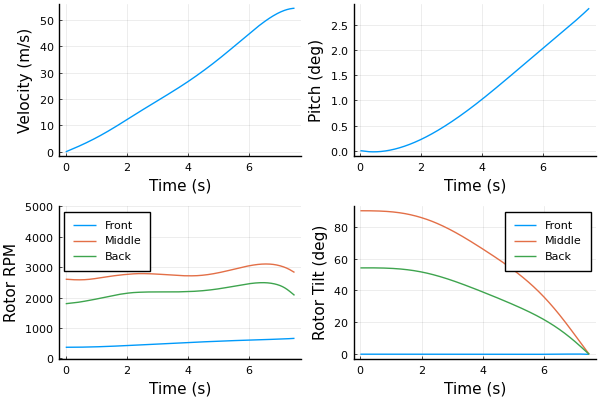
\includegraphics[width=0.8\textwidth]{figures/trajectory.png}
\caption{}
\label{fig:trajectory}
\end{figure}

As part of this study, we compare the force predictions from the VPM with those of a lower fidelity vortex lattice method (VLM) and show that the VLM does predict the correct trends, but does not capture the influence of a morphing wake during transition.  This discrepancy is shown in Fig. ~\ref{fig:comparison} where the two methods disagree by over 1000 N during early transition.

\begin{figure}[hbt!]
\centering
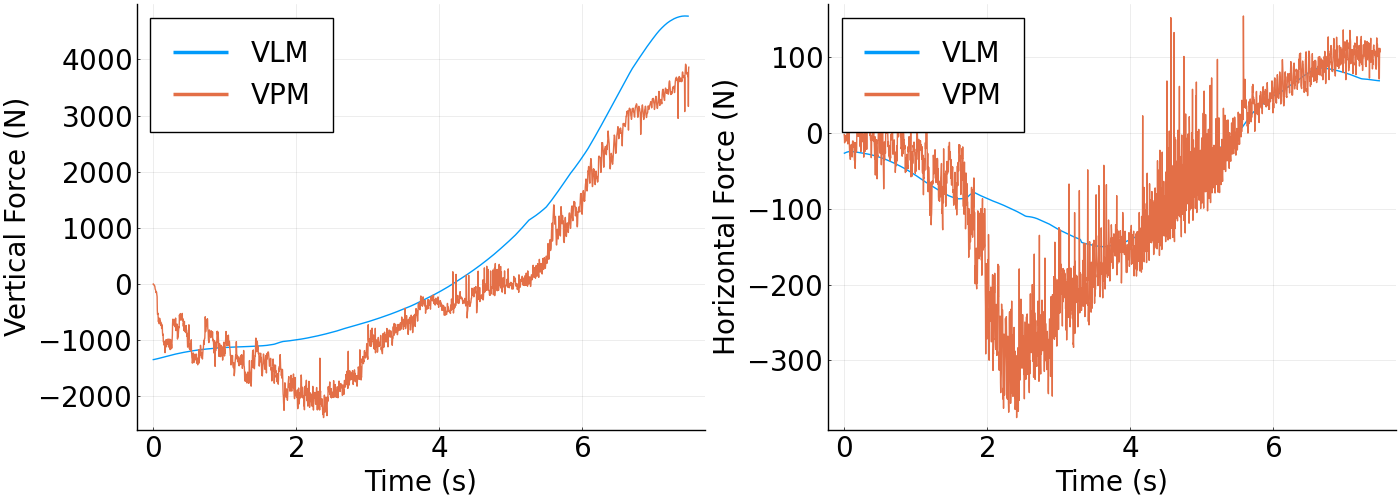
\includegraphics[width=0.9\textwidth]{figures/comparison.png}
\caption{}
\label{fig:comparison}
\end{figure}


\subsection{Neural time step reduction}

The techniques outlined above present a feasible approach to trajectory optimization in the VPM by overcoming key challenges such as noise and the high cost of derivatives.  However, the above optimization took roughly 428 hours to complete, which is a major limitation on the practicality of this approach. To address this issue, we will present a novel methodology that aims to accelerate the VPM by reducing the time steps necessary to solve the governing differential equations.  While a major motivation of this method is directed toward accelerating the VPM, it is completely general and can be applied to any ordinary differential equation (ODE).

Consider a general system of ODEs

\begin{equation}
    \frac{d\mathbf{x}}{dt} = f(\mathbf{x})
\end{equation}

If the dynamics of the system are fast, then small time steps will be necessary to resolve the correct trajectory, and if they are slow, then larger time steps may be sufficient, and we can simulate accurately with fewer of them.

The best metric for determining whether the dynamics are fast or slow is the spectral radius of the system's Jacobian, defined as

\begin{equation}
    \rho\left(\frac{df}{d \mathbf{x}}\right) = ||\boldsymbol{\lambda}||_{\infty}
\end{equation}

where $||\boldsymbol{\lambda}||_{\infty}$ is the magnitude of the largest eigenvalue of $\frac{df}{d\mathbf{x}}$

We desire a dynamic system which has a small spectral radius, and therefore slow dynamics, so that we can simulate the system accurately with only a small number of time steps.  To achieve this, we will leverage two neural networks $\phi$, and $\psi$ that together form an autoencoder pair.

\begin{equation}
    \mathbf{z} = \phi(\mathbf{x}) \quad \mathbf{x} = \psi(\mathbf{z})
\end{equation}

where $\mathbf{z} \in \mathbb{R}^m$ is a learned latent space, and is of higher dimension than $\mathbf{x} \in \mathbb{R}^n$:  $m > n$. 

Then, by the chain rule,

\begin{equation}
    \frac{d\mathbf{z}}{dt} = \frac{d \phi}{d \mathbf{x}} \frac{d \mathbf{x}}{dt} 
\end{equation}

Both $\frac{d \phi}{d \mathbf{x}}$ and $\frac{d \mathbf{x}}{dt}$ are functions of $\mathbf{x}$, but we can substitute $\mathbf{x} = \psi(\mathbf{z})$ to obtain

\begin{equation}
    \frac{d\mathbf{z}}{dt} = \frac{d \phi}{d \mathbf{x}} \left( \psi(\mathbf{z}) \right) \frac{d \mathbf{x}}{dt}\left( \psi(\mathbf{z}) \right) 
\end{equation}

We have now expressed the dynamic system entirely in $\mathbf{z}$ space, and it is completely general because it was derived from the known dynamics of the system and the chain rule. 

The next step is to train $\phi$ and $\psi$ to enforce slow dynamics in the latent representation. We define a loss function to be the spectral radius of the new dynamic system's Jacobian. 

\begin{equation}
    L_d = \rho\left( \frac{d \dot{\mathbf{z}}}{d \mathbf{z}} \right) 
\end{equation}

If we want the dynamics to be slow over a large domain in $\mathbf{z}$ space, then we need to penalize the spactral radius of the Jacobian at many points $\mathbf{z}_k$ in that domain

\begin{equation}
    L_d = \frac{1}{N} \overset{N}{\underset{k=0}{\sum}} \rho\left( \frac{d \dot{\mathbf{z}}}{d \mathbf{z}} \Big|_{\mathbf{z}_k} \right) 
\end{equation}

The other loss function that we need to define is the standard autoencoder reconstruction loss to ensure that we learn a valid latent representation

\begin{equation}
    L_r = \frac{1}{N} \overset{N}{\underset{k=0}{\sum}} ||\mathbf{x}_k - \psi(\phi(\mathbf{x}_k))||_2^2
\end{equation}

The autoencoder pair is then trained to minimize the combined loss function

\begin{equation}
        \underset{\phi, \psi}{\text{minimize}} \; \; \; \; \frac{1}{N} \overset{N}{\underset{k=0}{\sum}}\rho\left( \frac{d \dot{\mathbf{z}}}{d \mathbf{z}} \Big|_{\mathbf{z}_k} \right) + ||\mathbf{x}_k - \psi(\phi(\mathbf{x}_k))||_2^2 
\end{equation}

This method has been shown to be successful in reducing the number of time steps necessary to simulate the following ODE

\begin{equation}
    \frac{dx}{dt} = -15x
\end{equation}

which has eigenvalue $\lambda = -15$.  Because the dynamics are relatively fast, a time step of $0.01$ was necessary to accurately simulate the trajectory using euler integration.  An autoencoder was trained using the above loss function, and then simulated accurately with a time step of $0.1$ - an order of magnitude larger than what was required for the original system.  As shown in Fig. ~\ref{fig:neural_time_steps} we simulated this new system and then reconstructed the original states using the decoder network.  The new system was shown to perform much better than the original system when using a large time step of $0.1$

\begin{figure}[hbt!]
\centering
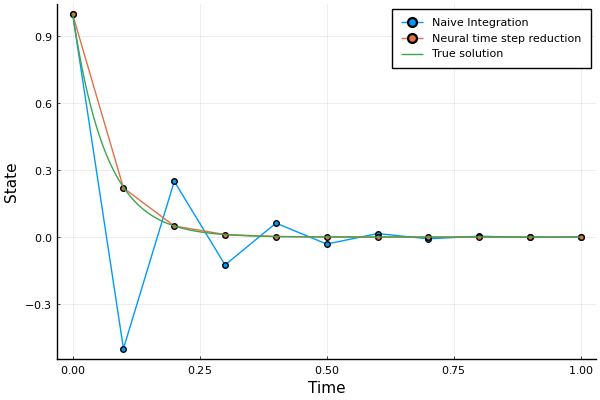
\includegraphics[width=0.8\textwidth]{figures/neural_time_step.png}
\caption{}
\label{fig:neural_time_step}
\end{figure}

\subsection{Koopman learning}

The neural time step reduction method described above has the potential to significantly speeed up VPM simulations, and enable their use in iterative optimization loops.  However, on its own, neural time step reduction is unlikely to achieve the speedups necessary for real time control, which requires many full simulations every second.  In order to facilitate real time VPM-based control, we seek linear models that can be used to solve the optimal control problem analytically. 

In order to achieve this, we leverage Koopman operator theory, which states that for any dynamic system

\begin{equation}
    \frac{d \mathbf{x}}{dt} = f(\mathbf{x})
\end{equation}

there exists a mapping $\mathbf{z} = \phi(\mathbf{x})$ such that 

\begin{equation}
    \label{eq:Koopman}
    \frac{d\mathbf{z}}{dt} = K \mathbf{z}
\end{equation}

where $K$ is the Koopman operator and represents the globally linear dynamics of $\mathbf{z}$ space. Koopman operator theory states that such a map exists, but that it is potentially infinite dimensional. 

To overcome this challenge, most current approaches apply machine learning to learn a finite dimensional approximation to the Koopman operator.  For the mapping $\mathbf{z} = \phi(\mathbf{x})$ one can use existing basis functions like Hermite polynomials, but it's generally better to train a neural network to learn the best mapping possible.

Because current methods typically rely on trajectory data simulated or experimentally obtained beforehand, there is always a risk of overfitting to the specific trajectories in the data set.  Because of this we are pursuing multiple options to potentially improve the generality of the Koopman learning process.

\subsubsection{Method of characteristics}

One way to approach learning the linear Koopman dynamic system is by considering the set of partial differential equations that arise from applying the chain rule to the learned latent space.

\begin{equation}
    \frac{d \mathbf{z}}{dt} = \frac{d \mathbf{z}}{d \mathbf{x}} \frac{d \mathbf{x}}{dt} = \frac{d \mathbf{z}}{d \mathbf{x}} f(\mathbf{x})
\end{equation}

Setting this equal to \ref{eq:Koopman} gives

\begin{equation}
    \frac{d \mathbf{z}}{d \mathbf{x}} f(\mathbf{x}) = K \mathbf{z}
\end{equation}

which is a linear partial differential equation that an be routinely solved using the method of characteristics.  The method of characteristics solves for $z$ along characteristic curves by reducing the problem to a set of ordinary differential equations parameterized by a variable $t$

\begin{equation}
    \frac{d\mathbf{x}}{dt} = f(\mathbf{x}), \; \;
    \frac{d\mathbf{z}}{dt} = K \mathbf{z}
\end{equation}

This is the expected result and tells us that as $\mathbf{x}$ evolves according to $f(\mathbf{x})$, $\mathbf{z}$ evolves according to $K \mathbf{z}$.  By itself, this is not useful yet because in order to solve for $\mathbf{z}$ we need to simulate the original dynamic system.

We can go further by solving the $\mathbf{z}$ ODE analytically as a function of $t$

\begin{equation}
    \mathbf{z} = e^{Kt}\mathbf{z}_0
\end{equation}

where $\mathbf{z}_0$ is the initial condition.  Ideally we would like to solve for $\mathbf{z}$ as a function of $\mathbf{x}$ rather than $t$, but due to the nonlinearity of the system, we cannot solve for $t(\mathbf{x})$ analytically.  Instead, we propose approximating $t(\mathbf{x})$ using a neural network.  This acts as a "time-to-reach" function, predicting how long it takes to reach a certain point in $\mathbf{x}$ space from a given initial point.

$t(\mathbf{x})$ alone only applies along a specific trajectory.  In order to describe the full solution, we also need to identify which trajectory a point belongs to.  To address this, we introduce another scalar valued network $l(\mathbf{x})$ to act as a "label" for each trajectory.  Given a point in $\mathbf{x}$ space, $l(\mathbf{x})$ identifies which trajectory we are on, and $t(\mathbf{x})$ tells how far along that trajectory we are.

With these two functions defined, we have

\begin{equation}
    \mathbf{z} = e^{Kt(\mathbf{x})}\mathbf{z}_0(l(\mathbf{x}))
\end{equation}

where $\mathbf{z}_0$ is a function that accepts the trajectory label and returns the initial conditions in $\mathbf{z}$ space.  This can be any function, but it should be injective to ensure unique initial conditions for each label value.

For training, we aim to find $t(\mathbf{x}$ and $l(\mathbf{x})$ satisfying

\begin{equation}
    \begin{matrix}
        \nabla t^T f(\mathbf{x}) = 1 \\
        \nabla l^T f(\mathbf{x}) = 0
    \end{matrix}
\end{equation}

In other words, $t$ increases unitarily along the trajectories, and $l$ is constant along the trajectories.  

If initial conditions are known we can also apply boundary conditions.  If $\mathbf{x}_0$ defines all the initial conditions, then we can enforce

\begin{equation}
    \begin{matrix}
        t(\mathbf{x}_0) = 0 \\
        l(\mathbf{x}_0) = \omega(\mathbf{x}_0)
    \end{matrix}
\end{equation}

where $\omega(\mathbf{x}_0)$ is a known function defining the trajectory labels.  For example, if $\mathbf{x} = (x, y)^T$ and we define initial conditions along the line $x = 0$, then the boundary conditions are $t(0,y) = 0$ and $l(0,y) = y$.  This means that trajectories start on the $y$-axis, and are labeled by their $y$ value.

This method was used to learn a solution to the Koopman problem for a simulated glider undergoing a transient maneuver before stabilizing.  The results where compared to the standard method of simply defining a vanilla neural network for $\mathbf{z}(\mathbf{x})$.  In both methods, the latent states were simulated from initial conditions using the learned Koopman operator $K$, and compared to their "true" values which where encoded directly from the original trajectory.  As shown in Fig. ~\ref{fig:method_of_characteristics}, the method of characteristics approach outperforms the standard method for the same number of collocation points.  

\begin{figure}[hbt!]
\centering
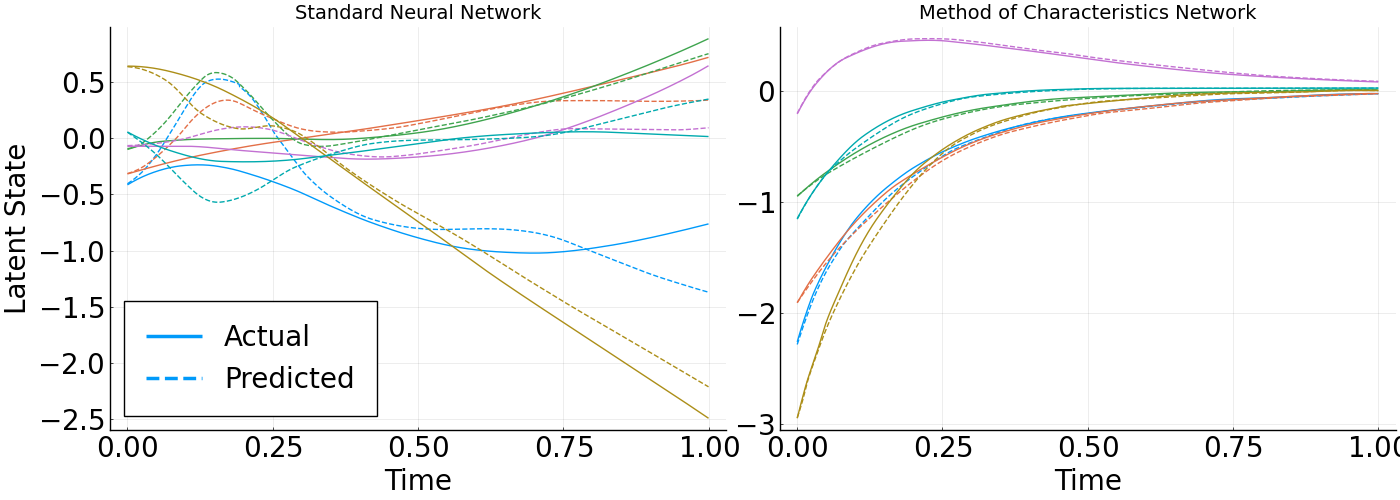
\includegraphics[width=0.9\textwidth]{figures/method_of_characteristics.png}
\caption{}
\label{fig:method_of_characteristics}
\end{figure}

\subsubsection{Projection onto a neural basis}

Leveraging the method of characteristics is potentially more genearlizable than the current state of the art in Koopman learning, but it still relies on obtaining trajectory data, and may be subject to overfitting.  Therefore we pursue a secondary approach directed toward constructing the Koopman operator without relying on data at all.

Given a set of basis functions $\phi_n(\mathbf{x})$ we can can represent a function $f(\mathbf{x})$ by an expansion in the basis

\begin{equation}
    f(\mathbf{x}) = \overset{\infty}{\underset{n=0}{\sum}} a_n \phi_n(\mathbf{x})
\end{equation}

where $a_n$ is the projection of the function onto the $n$th basis over the domain of interest

\begin{equation}
    a_n = \int_D f(\mathbf{x}) \phi_n(\mathbf{x})  d \mathbf{x}
\end{equation}

The Koopman operator can be thought of a matrix of these projection values.  If we have the discrete dynamic system $\mathbf{x}_{k+1} = F(\mathbf{x}_k)$, we want to find a matrix $K$ such that 

\begin{equation}
    \phi(\mathbf{x}_{k+1}) = \phi(F(\mathbf{x}_k)) = K \phi(\mathbf{x}_k)
\end{equation}

So we need to construct the function $\phi(F(\mathbf{x}_k))$ by an expansion in the basis $\phi(\mathbf{x}_k)$.  The Koopman operator $K$ is therefore a projection of the desired function onto this basis

\begin{equation}
    \label{eq:koopman_projection}
    K_{ij} = \int_D \phi_i(F(\mathbf{x})) \phi_j(\mathbf{x})  d \mathbf{x}
\end{equation}

This construction is desireable because it does not rely on data at all, and instead gives an analytic form of the best possible Koopman operator for a given set of bases.  

There are two main challenges of this approach.  The first is that the basis functions $\phi_n$ may not be the ideal basis for expressing the underlying dynamics, which could lead to large errors unless $\phi_n$ is infinite.  

To address this issue, we will define $\phi_n$ as a neural network and train it to learn the best possible basis to work in for the specific problem.  As a measure for how good the basis is, we examine the values of the projection coefficients, which reveal how much of the original function was captured by the projection.  This is mathematically expressed through Parseval's theorem which states that for the expansion of a function $f(x)$ a complete basis,

\begin{equation}
    ||f||^2 = \overset{\infty}{\underset{n = 0}{\sum}} |a_n|^2
\end{equation}

If this relation is true, then all of the "energy" of the function $f(x)$ is captured in the coefficients, and the function is exactly reconstructed.  Applied to the Koopman problem, this means we can define a loss function

\begin{equation}
    L_i = ||\phi_i(F(\mathbf{x}))||^2 - \overset{N}{\underset{j = 0}{\sum}} |K_{ij}|^2
\end{equation}

Minimizing this error over all the rows of the Koopman operator will yield the best possible basis.

The second big challenge is that the integrand $\phi_j(\mathbf{x}) \phi_i(F(\mathbf{x}))$ from \ref{eq:koopman_projection} is potentially a very nonlinear and complex function that cannot be integrated analytically.  We can integrate numerically over the domain, but if the $\mathbf{x}$ is high dimensional, this quickly becomes extremely expensive.

We address this issue by recognizing that any complex function $f(x)$ can be described by a computational graph which consists of the composition of many simple operations $f(x) = f_n \circ \cdots \circ f_3 \circ f_2 \circ f_1 \circ x$.  

Finding the projections for just $f_1$ is potentially easier if $f_1$ is a simple operation

\begin{equation}
    \phi(f_1(x)) = K_1 \phi(x)
\end{equation}

Then, if we find the projections for $f_2$, 

\begin{equation}
    \phi(f_2(x)) = K_2 \phi(x)
\end{equation}

we can construct the projections for $f_2 \circ f_1$ because we have

\begin{equation}
    \phi(f_2(f_1(x))) = K_2 \phi(f_1(x)) = K_2 K_1 \phi(x)\\ 
\end{equation}

We can therefore construct the full Koopman operator of $f$ by

\begin{equation}
    \phi(f(x)) = K_n \cdots K_2 K_1 \phi(x) = K \phi(x)\\ 
\end{equation}

This approach has the potential to be arbitrarily general because we relied on projection of our function onto a custom basis instead of training data.  However, it is currently only in the very early stages of development and remains untested.  It is also possibly susceptible to very large errors because each projection is an approximation, and the error accumulated over a large computational graph can be very significant unless it is trained sufficiently to minimize that error. For this reason, we will pursue both the projection approach and the method of characteristics approach to achieve the best outcome.


\section{Anticipated Contributions}


The proposed work, as outlined in the previous section, aims to bridge the gap between high fidelity simulation, and iterative optimization and control applications through several key contributions:

\begin{enumerate}
\item A practical demonstration of VPM-based trajectory optimization, including a comparative analysis that underscores the importance of unsteady modeling during eVTOL transition phases.
\item The development of a neural time-step reduction methodology applicable to any general set of ODEs, which will substantially accelerate high-fidelity simulations while preserving accuracy.
\item An enhancement of the generalizability of the Koopman learning process, enabling more robust linearization of nonlinear dynamics and supporting real-time control of complex, high-fidelity systems.
\end{enumerate}

Together, these efforts will create a cohesive framework that unites high-fidelity aerodynamic modeling, machine learning, and control theory. By overcoming the computational and modeling barriers that have traditionally separated simulation from real-time decision making, this research will make it possible for optimization and control algorithms to directly leverage unsteady aerodynamic effects. In doing so, it lays the foundation for a new generation of aircraft design and control strategies—ones that are not only faster and more efficient, but also fundamentally more adaptive and aware of the physics that govern their motion.




% Why will it matter when you succeed
    % Optimization of aircraft that go through unsteady maneuvers will be more accurately informed
    % Control of unsteady maneuvers will be more reliable and safer
    % Other fields will benefit from general improvements to ODE simulation and Koopman learning

% Scientific contributions

% Methodological contributions

% Practical impact

 


\pagebreak

\bibliographystyle{IEEEtran}
\bibliography{library}

\end{document}
